\cotefile{161-2}
\scanpage{51}
\inserted{(\unsure{?? sens|22 suit})}
\deleted{\unsure{S}}Soit $\Pi'_n=\bigcap\Pi_{nj}$, et $e'_n=\operatorname{Im}(\Pi'_n\mathbin{\unsure{-|\to}}e_E)$. La condition est que $e'_n\to e_E$ est un \uline{iso}, i.e. $\pi'_n\to 1_E$ un épi. Il n'est pas clair cependant que la formation des $e'_n$ commute aux chgt de topos de base $E'\mathbin{-}E$, car ce n'est pas clair pour la formation des $\Pi_{nj}$. Donc il n'est pas clair qu'on a un topos modulaire \deleted{\unsure{triplement}},

Mais prenons d'abord le \unsure{pbt|pbl|pts} analogue des anneaux qui sont \uline{de plus} de support tout.
\margin{\uline{lemme} \uline{à vérifier}}% slanted
Alors on voit que localement le choix des $e_i$ est bien déterminé, \deleted{\unsure{à cela près|à cette fois}} à permutation près, et de plus que si \deleted{\unsure{on a un}} on désigne localement par $m$ le nb de $e_i$ qui sont $\ne 0$, alors \deleted{la décomposition} les $e_i$ sont tous \deleted{\unsure{à}} \unsure{différent|différents} (\unsure{et|c'est} pour cause, $e_i=e_j$ \unsure{et} $e_i^2=e_i$, $e_i e_j(=e_i^2)=0$ implique $e_i=0$!) Si on se borne pour le moment au cas où $n=m$, on trouve que \deleted{le choix des} \deleted{\unsure{le}} faisceau des choix possibles des \deleted{$\unsure{e}$} $e_i$ est un pseudo-torseur \inserted{sur $E$} sous le groupe \inserted{symétrique} $\unsure{\mathfrak S|\mathscr S}_n$; dire \deleted{que} \deleted{est} $A$ est \inserted{quasi} connexe de rang \uline{exact} $n$, (ce qui implique, par définition, à support \deleted{\unsure{et $\ne$}} tout). \deleted{\unsure{Ceci}}

Je ne sais si les \uline{pseudo}-\uline{torseurs} commutent à tt chgt de base \inserted{$\unsure{E'|E_i'}\mathbin{-}E$}, mais le torseur oui, si on se borne aux $E$ munis de $A$ quasi-connexe de rang exact $n$. Or la donnée d'un tel revient à la donnée

a) d'un $\mathfrak S_{n\,E}$-torseur $P$ (sur $E$, i.e. d'un morphisme $E\xrightarrow{p}B_{\mathfrak S_n}$ (\unsure{ou plus de|ou plus des} $E\to\widehat R=B)$,

b) d'une décomposition de $A_P$ en produit $\prod_{1\le i\le n} A_i$ avec les $A_i$ connexes (néc. à support tt), et avec compatibilité entre celle-ci et l'action de $\mathfrak S_n$.

Cela signifie qu'on a le torseur $P$ (i.e. $p$), des anneaux connexes \deleted{\unsure{non}} à support tout $A_i$ situés sur $P$, et \deleted{\unsure{une}} action de $\mathfrak S_n$ sur $P$ permutant \unsure{entre eux|avec} les $A_i$ suivant des actions sur les indices.
% archive sheet number: 50
\scanpage{52}
$M$ \uline{plat} cela est-il une propriété typique [elle est stable par $\varinjlim$ \unsure{filtr|filtr.} et par chgt de topos $\}$

\[
 N\longmapsto M\otimes N\quad\text{exact}
\]
$\forall\ f_1$ -- $f_n$ sections de $A$ sur $U$,
\[
 (\textstyle\sum f_i A)\otimes M\longrightarrow M\quad\text{injectif}
\]
Il suffit de l'exiger \deleted{pour} les \inserted{\unsure{syst. de}} sections \unsure{universel|universelles}, i.e. $U\unsure{:=|=} A^n$
\[
 (\textstyle\sum t_i A_{U_n})\otimes M_{U_n}\longrightarrow M_{U_n}\quad\text{injectif.}
\]
\[
 U_n=A^n
\]
\diagram{\begin{tikzcd}[ampersand replacement=\&,column sep=small,row sep=small]
 M\arrow[d,dashed,no head]\arrow[r,dashed] \& M_i\\
 Y\arrow[dr] \& Y_i\arrow[l]\\
 \& N,\text{ plat}\\
 Z\arrow[uu,bend left=18] \&
\end{tikzcd}
\qquad
\begin{tikzcd}[ampersand replacement=\&,row sep=small,column sep=small]
 M\arrow[r] \& \unsure{M'|M_i} \&\\
 A\arrow[r]\arrow[drr,no head] \& \unsure{A'|A_i} \& N\,\text{plat}\arrow[d,no head]\\
 \& \& B
\end{tikzcd}}

\diagram{\begin{tikzcd}[ampersand replacement=\&]\mathbf Y\&\mathbf X\arrow[l]\end{tikzcd}}

\figure{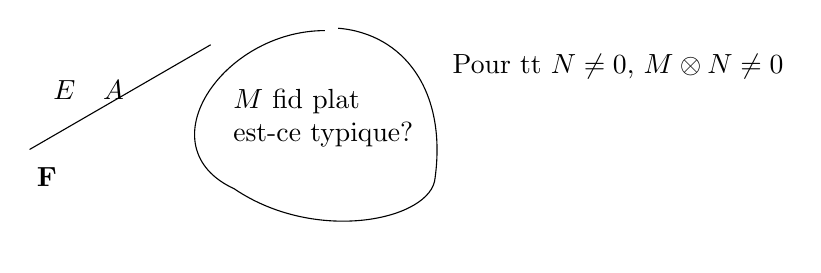
\begin{tikzpicture}
\node at (0,.2) {$E\quad A$};\draw (-.75,-.55) -- (1.55,.78);
\node at (-.53,-.9) {$\mathbf F$};
\draw (3,.96) .. controls (1.7,.96) and (.7,-.52) .. (1.85,-1.05) .. controls (2.9,-1.76) and (4.36,-1.44) .. (4.4,-.91) .. controls (4.55,.2) and (4,.92) .. (3.17,.99);
\node[align=left] at (2.98,-.15) {$M$ \uuline{fid} \uline{plat}\\est-ce typique?};
\node[anchor=west] at (4.5,.5) {Pour tt $N\ne 0$, $M\otimes N\ne 0$};
\end{tikzpicture}}

$\mathbf E_{\mathbf A}$\qquad \uuline{Modpf} $(A)$ champ des modules de p.f. sur $A$
\[
 \underline{\operatorname{Hom}}\bigl(\text{\uuline{Modpf}}(A),\text{\uuline{Fl}}(E)\bigr)
 \qquad\text{Catégorie des hom de Champs \unsure{de|des}}
\]
\deleted{les objets}
\[
 \begin{aligned} E&\longrightarrow F& &\text{hom. de champs \uline{constants}}\\
 &&M&\longmapsto X \end{aligned}
\]
d'où \quad $A_{\mathbf F}$ \qquad $\mathbf R$

\uline{Algèbres}
\diagram{$\displaystyle\left.\begin{array}{l}
 \text{\deleted{de} t.f}\\ \text{p.f.}\\ \text{lisses}\\ \text{étales}\\ \text{nettes}
 \end{array}\right]\quad
 \begin{array}{l}\text{\unsure{$\leftarrow$}}\\\text{peu typiques}\\\text{car ne \unsure{commut|commutent} pas}\\\text{aux }\underrightarrow{\lim}\end{array}$}

\diagram{$\left|\begin{array}{ll}
 \text{\uline{radicielles} / monomorphiques} & \deleted{\unsure{\rm OK}}\ \text{OK, par prod. fibrés.}\\
 \boxed{\text{\uline{surjectives} \unsure{?|X|?!}}} &\\
 \text{plates}^{\text{OK}}\text{ / fid plates}&\\
 \text{formellmt lisse}&\\
 \text{--- net}&\text{OK}\\
 \text{--- étale}&\\
 \text{entières}&\text{OK}\\
 \text{homéo. universels}&
 \end{array}\right.$}

\margin{Considérons une Algèbre qui est déjà de \uuline{\deleted{\unsure{t}}p.f.} On veut ``la \unsure{vendre|rendre}'' plate, ou lisse etc. Cela se fait-il par un sous-topos ??}
% archive sheet number: 51
\scanpage{53}
\margin{\uline{propriétés} \uline{non topiques} \inserted{(pour topos)} absolues pour anneaux $\left\{\begin{array}{l}\text{artinien, noethérien, de t.f. sur $\mathbb Z$ (ou sur}\\ \text{$n$ composantes connexes\qquad $\unsure{\mathbb Q|Q}$, \deleted{\unsure{ou sur}}}\\ \text{$n$ composantes irréductibles\qquad ou $\mathbb Z S^{-1}\ldots$)}\end{array}\right.$}

\deleted{\uline{Propriétés relatives d'anneaux}}

Anneaux plongeables dans des corps : il \uline{faut} qu'ils soient intègres,
\margin{(voir anneau \unsure{hensélien}, ou ---- \unsure{hens\ldots})}
mais ce n'est pas suffisant \inserted{même s'il est local \unsure{hensélien|hypothèse}}. Pour l'anneau intègre universel, les sections locales qui sont partout non nulles (donc qui sont $A$-régulières) sont celles qui sont inversibles : l'anneau total des fractions \deleted{\unsure{doit}} est égal à $A$ lui-même. Une condition nécessaire pour qu' \deleted{\unsure{A soit un}} un Anneau se plonge \unsure{$\to X$|$X'\to X$} dans un corps, c'est que la section nulle (donc tte autre section) soit \unsure{sommande|sommante} direct de $A$, et c'est sans doute suffisant

\uline{Modules sur anneau}
\[
 X_{\mathrm{mod}}=\widehat{\mathit{Mod}^{\circ}_{pf}}
\]
\[
 \begin{aligned}\mathit{Mod}_{pf}&=\text{catégorie des modules de prés. finie sur $\mathbb Z$-algèbres de prés finie $\unsure{\in|\mathscr E}$}\\
 \mathit{Mod}_{pf}^{\circ}&\simeq\text{\deleted{schémas} Modules \deleted{\unsure{fibrés}} sur schémas affines de t.f. sur $\mathbb Z$.}
 \end{aligned}
\]
\diagram{\begin{tikzcd}[ampersand replacement=\&,row sep=small]
 M\arrow[r]\arrow[d,no head]\&N\arrow[d,no head]\\
 A\arrow[r]\&B\\
 \mathscr F\&\mathscr G\\
 Y\& X\arrow[l]
\end{tikzcd}}
\diagram{$\begin{array}{l}
 \left\{\begin{array}{l}\text{Localement libre}\\ \text{libre, projectif / injectif (?)}\end{array}\right.\\
 \left\{\begin{array}{l}\text{localemt libre de rang $n$}\\\text{libre de rang $n$}\end{array}\right.\quad(n\geq 1)\\
 \text{\unsure{ou|$n$}}\\ \text{de \unsure{t.f.|N.f.}}\\ \text{de prés finie}\\ \text{monogène}
 \end{array}$}
\margin{ne passent pas à la limite inductive ? donc pas topiques}% slanted

\deleted{\unsure{Plats, libres, projectifs}}
\[
 M\ \text{inv.}\quad\Longleftrightarrow\quad M\otimes_A\underbrace{\underline{\operatorname{Hom}}_A(M,A)}\xrightarrow{\sim}A
\]
\margin{n'est pas exprimable par \unsure{lim|les lim|$\varinjlim$} / ne commute pas au chgt de base du \unsure{sg}}% slanted

\deleted{\unsure{$\exists$|$\exists N$} $M\otimes N\simeq A$ \quad $X\longmapsto M\otimes X$\quad $\unsure{\operatorname{Hom}(X,Y)\simeq\operatorname{Hom}(TX,TY)|\underline{\operatorname{Hom}}(X,Y)\to\underline{\operatorname{Hom}}(f^*X,f^*Y)}$\quad $\unsure{\operatorname{Hom}(T'TX,T'Y)}$}

\deleted{\unsure{$F(M\otimes$}$\,\unsure{N)}$ \quad \unsure{$T_M T_N\simeq 1\Longrightarrow$} \unsure{$\mathcal U$} \quad $T_M T_N\simeq\mathrm{id}$\quad donc $T_N,T_M$ des équivalences\quad $\unsure{\operatorname{Hom}(X,Y)|\underline{\operatorname{Hom}}(X,Y)}$}

\deleted{\unsure{mor} $M'\to M$ et $M\otimes P\to M\otimes Q$\quad $T_N T_M\simeq\mathrm{id}$\quad donc exacts,}

\deleted{donc $M$ et $N$ \inserted{fid} plats. $M=\lim M_i$, les $M_i\subset M$ de t.f., donc $A\simeq M\otimes N=\underset{\longrightarrow}{\lim}\,M_i\otimes N$, donc $M_i\otimes N\subset A$, donc $\unsure{\exists}$ on a $M_i\otimes N=A$ pour \unsure{$i$|$A'$|$A$} grand, donc $M_i=M$, donc $M$ de t.f., \deleted{\unsure{Il est}} $N$ pareil. $M$ est monogène}
% archive sheet number: 52
\scanpage{55}
\uline{Catégories $\operatorname{Ind}$}$_\pi(C)$ ($\deleted{\unsure{\pi}} C$ petite) et $\deleted{\operatorname{Ind}_\pi(C)_{\pi'}\unsure{(\mathscr E)}}\operatorname{Fil}^{\pi}(\operatorname{Ind}_{\pi}(C))$

\uline{Th.} $E$ \inserted{$\mathcal U$-}catégorie [stable par petites $\varinjlim$ ? \inserted{ou satisfaisant seulement $L_\pi$ ?}]. Conditions équivalentes

a) $E$ $\pi$-accessible

b) $E$ équivalente à une catégorie $\operatorname{Ind}_\pi(C)$, $C$ petite

c) La sous-catégorie $E_\pi$ de $E$ formée des objets $\pi$-accessibles est équiv. à une petite cat. et elle est strictement génératrice.

\deleted{et de même une filtration ordinale, si $\pi'\geq\pi$ \unsure{cf hypothèse} $\pi'\geq\pi$.}

Sous ces conditions, \deleted{$E$ admet une filtration \unsure{ordinale|cardinale}, $(\unsure{E^\circ_\pi}(E_\pi))_{\pi'\geq\pi}$} on a $E_{\pi'}\simeq\unsure{\operatorname{Ind}}(\operatorname{Ind}_{\pi}(E_\pi)_{\pi'})$, et les $(E_{\pi'})_{\pi'\geq\pi}$ forment une filtration ordinale
\deleted{\unsure{de filtration}}.

Préciser la filtration ordinale \deleted{\unsure{de|des}} $(\underline{\operatorname{Fil}}^{\pi})_{\pi\geq\pi_0}$ \unsure{---}
\[
 \operatorname{Fil}^{\pi'}(E)=E_{\pi'}\inserted{{}=\operatorname{Ind}_{\pi}(C)_{\pi'}}\quad\text{pour $\pi'$ grand,}
\]

\uline{Cor} Soient $E$ et $F$ deux catégories accessibles, \inserted{donc $E\simeq\operatorname{Ind}_\pi(E_\pi)$, $F\simeq\operatorname{Ind}_\pi(F_\pi)$ pour $\pi\geq\pi_0$ \deleted{gd}} \deleted{Alors} $f:E\to F$ un foncteur. \deleted{Alors} Conditions équiv..

a) $f$ est \deleted{$\pi$-}accessible \deleted{\unsure{c)}} b) $\exists\ \pi$ tel que $f\simeq\operatorname{Ind}_\pi(f_\pi)$, où $f_\pi:E_\pi\to F_\pi$ un foncteur. \deleted{[et pour un tel $\pi$, $f$ est $\pi$-accessible]. Preuve que} [Pr. v. que pr $\pi$ canonique, il $f$ est \unsure{''} que $f$ soit $\pi$-accessible et envoie $E_\pi$ dans $F_\pi$]. c) $\exists$ une petite sous-catégorie pleine $C$ de $E$, $i:C\to E$ telle que $f$ soit dans l'image essentielle de $i_!^F$ :
\deleted{b) Pour un tel $\pi$, $\unsure{i|f_i}$ est} $\underline{\operatorname{Hom}}(C,F)\to\underline{\operatorname{Hom}}(E,F)$.

\uline{Corollaire} Supposons $f$ $\pi$-accessible. Alors \deleted{\unsure{il y a}} $\exists\ \pi_0$ tel que
\[
 \pi\geq\pi_0\Longrightarrow f(E_\pi)\subset F_\pi .
\]
\margin{\uline{Corollaire} \inserted{$E$ $\pi$-accessible, $F$ qlc. Alors} $\underline{\operatorname{Hom}}(E,F)_\pi\overset{\deleted{\unsure{\sim}}}{\longrightarrow}\underline{\operatorname{Hom}}(E_\pi,F)$ pl. fid, c'est une équivalence de catégories \deleted{\unsure{ssi}} si $F$ satisfait $L_\pi$}

\uline{Th} Soit $C$ une catégorie accessible \inserted{avec petites $\varinjlim$.} \deleted{\unsure{$f$:}} Alors

a) (Pour mémoire) les foncteurs contravariants $C^\circ\to(\mathrm{Ens})$ repr. sont ceux qui commutent aux \inserted{petites} $\varinjlim$\deleted{\unsure{---}}

\margin{8.13.2 $(+8.12.8.1)$}

b) Un foncteur covariant \deleted{\unsure{en}} $C\to(\mathrm{Ens})$ est proreprésentable \inserted{(resp.)} \deleted{ssi $\unsure{\Pi|\pi}$ est accessible et} \inserted{ssi il est} exact à gauche (resp. commute aux petites $\varprojlim$) et \uline{accessible}

\uline{Corollaire} Soit $f:C\to C'$ un foncteur, avec $C$ accessible \inserted{stable par petites $\varinjlim$}.

a) $f$ admet un adjoint à droite ssi $f$ commute aux \inserted{petites} $\varinjlim$

b) $f$ admet un \inserted{pro}adjoint \deleted{\unsure{en}} (resp. un adjoint) à gauche ssi il est exact à \unsure{g} (resp. commute aux \inserted{petites} $\varprojlim$) \deleted{que} et est \uline{accessible}.

\uline{Th.} a) Soit $E\to B$ une catégorie fibrée, avec $B$ équiv. à une \deleted{\unsure{petit|petite}} \inserted{petite} catégorie, les catégories fibres accessibles, les foncteurs changement de base accessibles. Alors $\varprojlim E/B$ et $\underline{\operatorname{Hom}}_B(B,E)$ sont accessibles. En particulier, si $C$ accessible et $I$ équiv. à une petite catégorie, $\underline{\operatorname{Hom}}(I,C)$ est accessible, ainsi que la sous-catégorie pleine des foncteurs qui transforment tte flèche en un iso.

\margin{9.22}

b) Même hyp. sur $E,B$. Alors $\varinjlim E/B^\circ$ est accessible.
\margin{à \unsure{voir|revoir|établir|vérifier} $\longrightarrow$}% slanted
% archive sheet number: 54
\scanpage{56}
% archive sheet number: 55
\margin{Ref à SGA4 I}

\uline{Catégories accessibles}

\deleted{\unsure{Catégorie filtrante}} \inserted{Ensemble \inserted{pré}ordonné} grand devant $\pi$. Conditions $L_\pi,L$

Foncteur $\pi$-accessible, accessible

Objet $\pi$-accessible, objet accessible d'une catégorie.
\margin{$9,1$ à $9.3$}

Catégorie $\pi$-accessible : Satisfait $L_\pi$, et admet une \inserted{petite} sous-catégorie \inserted{\uline{str.}} génératrice \deleted{telle que} \inserted{dont les} objets sont $\pi$-accessibles

\margin{(\unsure{modifié|vérifier} 9.4?) c'est la bonne notion si $E$ stable par petites $\varinjlim$; sinon les bonnes catégories sont les $\operatorname{Ind}_\pi(C)$ avec $C$ petite\ldots}% slanted

accessible : $\exists\ \pi$ tel que $C$ $\pi$-accessible

\margin{9.6}
\uline{Prop} \deleted{\unsure{Soit $f$ un fonct}} $\underline{\operatorname{Hom}}(E,F)_\pi$, $F$ satisfaisant $L_\pi$

a) stable par \inserted{les} $\varinjlim$ qui sont représentables dans $F$

b) Si $F$ $\pi$-accessible (faiblement) alors pour tte catégorie $J$ avec $\operatorname{card}\operatorname{Fl}J\leq\pi$ et les $\varprojlim$ de type $J$ repr. dans $F$, $\underline{\operatorname{Hom}}(\ )_\pi$ stable par $\varprojlim$ de type $J$.

\deleted{\unsure{Cor. 1 Hom}}

\uline{Cor 1} Cas \uline{accessible}

\uline{Cor 2} \deleted{\unsure{$E_\pi$ est}} Si $E$ est (fblt) \deleted{\unsure{$\pi$}} \inserted{$\pi$-}accessible, \deleted{\unsure{$E_\pi$ est}} pour tt $\pi'\geq\pi$, $E_{\pi'}$ est stable par $\varinjlim$ de type $J$, avec $\operatorname{card} J\leq\pi'$. [Les objets accessibles de $E$ stables par \inserted{petites} $\varinjlim$]

\uline{Cor 3} Si $E$ est accessible, tout objet de $E$ est accessible.

Réciproque \deleted{\unsure{à}} partielle : Si :

\margin{9.11}
\uline{Prop} \deleted{\unsure{Soit}} $E$ catégorie satisfaisant la condition $L$ et :
\deleted{a) $E$ admet une petite sous-catégorie str. gén.}

a) $E$ stable par noyaux de doubles flèches, et $\operatorname{Ker}$ est accessible (p.ex. commute aux \inserted{petites} $\varinjlim$ filtrantes)

b) $E$ stable par produits fibrés,

c) [\inserted{$E$ admet une petite sous-catégorie \deleted{\unsure{strictement|génératrice}} génératrice par épim. stricts universels} \deleted{Toute} famille épimorphique stricte est épim.\unsure{phique|plique} stricte universelle] \deleted{ou encore : les familles épimorphiques strictes sont épimorphiques strictes] ; i.e. si les familles épimorphiques sont épimorphiques strictes]}
\margin{($E$ admet une pet. ss-cat. str. génératrice, \uline{et} (p.ex}

Alors $E$ est accessible (id., en présence de a)) tout objet de $E$ est accessible

\deleted{\unsure{Conditions}}

[\uline{Cor} $E$ catégorie stable par petites $\varinjlim$, \deleted{et telle que, tte famille épimorphique stricte est épimorphique stricte universelle}

Conditions équivalentes

a) $E$ est accessible

b) $E$ admet une petite sous-catégorie \deleted{\unsure{str|génératrice}} génératrice \inserted{par épim. str. universels} \deleted{(comme} $E$ \deleted{\unsure{stable}} petites $\varprojlim$) et le foncteur Ker sur la catégorie des doubles flèches de $E$ est accessible.

\[
 \left[\ \underline{\mathrm{NB}}\quad E\text{ accessible}\Longrightarrow
 \left\{\begin{array}{l}
 \underline{\operatorname{Hom}}(C,E)\text{ accessible pour tte petite catégorie $C$}\,]\\
 \text{\deleted{\unsure{$E$|$\exists$}} ($E$ $\pi$-accessible) $E_\pi$ petite sous-catégorie gén. par épim.}\\
 \qquad\text{stricts universels}\,]
 \end{array}\right.\right.
\]

\uline{Ex.} \deleted{\unsure{D|Dans}} Un topos, \deleted{une catégorie opposée à un topos} une catégorie \deleted{abélienne} à $\varinjlim$ filtrantes exactes et à petite famille génératrice \deleted{l'opposée d'un} sont des catégories accessibles. Mais $(\mathrm{Ens})^\circ$ et $(\mathrm{Ab})^\circ$ ne sont pas accessibles, p.ex. \deleted{\unsure{$\exists$}} parce que dans ces catégories \deleted{\unsure{le fait que}} \deleted{il n'y a pas de \inserted{petite} sous-catégorie génératrice par épim. stricts universels} le $\operatorname{ker}$ n'est pas accessible [i.e. le foncteur coker dans Ens, (Ab) ne commute pas aux produits quelconque : une $\varprojlim$ grande devant $\pi$ d'épim n'est pas néc. un épim.]

\uline{Filtration cardinale} d'une catégorie $E$ \deleted{satisfaisant \unsure{$L$}} par des $\operatorname{Fil}^{\pi}(E)$, $\pi\geq\pi_0$

a) Les $\operatorname{Fil}^{\pi}(E)$ équivalents à petite catégorie

b) \deleted{\unsure{Que|Fil}} $E$ satisfait $L_{\pi_0}$, $\operatorname{Fil}^{\pi}$ stable par $\varinjlim$ filtrantes \deleted{grandes \unsure{au}} avec $I$ grand devant $\pi_0$ et $\operatorname{card}I\leq\pi$

\margin{9.12. (Condition c) renforcée)}
c) Si $\pi'\geq\pi\geq\pi_0$, tt élément $X$ de $\operatorname{Fil}^{\pi'}$ est de la forme $\varinjlim_{i\in I}X_i$. $X_i\in\operatorname{Fil}^\pi$, $I$ grand devant $\pi$, $\operatorname{card}I\leq\pi'$
\scanpage{57}
\diagram{\begin{tikzcd}[ampersand replacement=\&,column sep=small,row sep=small]
 C\arrow[rr,"\varphi"]\&\& E\\
 E\arrow[rr,"{}^a\varphi"]\arrow[dr,dashed,no head]\&\&\widehat C\\
 \&\widehat E\arrow[ur,dashed,"\varphi^*"']\&
\end{tikzcd}}
\[
 \operatorname{Hom}_E(\varphi(Y),X)\simeq\operatorname{Hom}_{\widehat C}(Y,{}^a\varphi(X))
\]
\[
 \begin{aligned}
 &\deleted{\unsure{\operatorname{Hom}_{\widehat E}(\varphi(Y),X)\simeq\operatorname{Hom}_{\widehat C}({}^a\varphi(X),Y)}}\\
 &\deleted{\unsure{\operatorname{Hom}_E(X,}}
 \end{aligned}
\]

Si ds $E$ $\exists$ \inserted{petites} limites inductives, on a aussi :
\[
 \bar\varphi:\widehat C\longrightarrow E\qquad
 \bar\varphi(F)=\varinjlim_{C/F}\varphi(X)
\]
\margin{la donnée de $\varphi$ équivaut à celle de $\bar\varphi$ commutant aux petites $\varinjlim$}
\[
 \operatorname{Hom}_{E}(\bar\varphi(F),X)\simeq\operatorname{Hom}_{\widehat C}(F,{}^a\varphi(X))
\]

\uline{Conditions équivalentes}
\[
 \left.\begin{array}{ll}
 \text{\textcircled{a}}&\forall X\in E,\quad\varinjlim_{Y\in C/X}\varphi(Y)\xrightarrow{\sim}X\\
 \text{\textcircled{b}}&{}^a\varphi:E\longrightarrow\widehat C\ \deleted{\unsure{\mathrm{est}|-}}\ \text{pl. fidèle}
 \end{array}\right\}\quad\text{On dit alors que $\varphi$ est strictement générateur.}
\]
b$'$) (Si $E$ stable par \inserted{petites} $\varinjlim$) $\widehat C\to E$ un foncteur de localisation [ou seulement : ess. surjct

\unsure{c$'$|b$''$|b$'$}) \deleted{\unsure{$\varphi E$}} (Si $E$ est stable par \inserted{petites} $\varinjlim$ filtrantes, et les $C/X$ ($X\in\operatorname{Ob} E$) filtrant, p.ex. $C$ stable par $\varprojlim$ finies et $\varphi$ exact à g :) : $\widetilde\varphi:\operatorname{Ind}(C)\to E$ induit par $\bar\varphi$ est une foncteur de localisation

c) (Si $\varphi$ admet un ind-adjoint, i.e. ${}^a\varphi$ prend ses valeurs dans $\operatorname{Ind}(C)$)
\[
 {}^{\mathrm{ia}}\varphi:E\mathbin{-}\operatorname{Ind}(C)\quad\text{est pl fidèle.}
\]

d) (si $\varphi$ admet un adjoint à droite $\psi$, i.e. ${}^a\varphi$ prend ses valeurs dans $C$)
\[
 \psi\ \text{est pl fidèle}
\]

d$'$) \deleted{$\varphi$ est un fonct\unsure{eur}} (\unsure{m\textsuperscript{e}|même} condition \inserted{que \unsure{f|d}}) $\varphi$ est un foncteur de localisation.

e) (si $\varphi$ pl. fidèle) $\varphi(C)$ est génératrice dans $E$ par épim. stricts.

\textcircled{f} Pour toute catégorie $F$ stable par petites $\varinjlim$, désignant par $\underline{\operatorname{Hom}}'(E,F)$ la sous-catégorie pleine de $\underline{\operatorname{Hom}}$ formée des foncteurs qui commutent aux petites $\varinjlim$, le foncteur restriction
\[
 \beta_F:\underline{\operatorname{Hom}}'(E,F)\mathbin{-}\underline{\operatorname{Hom}}(C,F)
\]
est pl. fidèle

\deleted{g') Avec les notations précédentes, le foncteur $\unsure{\alpha_F}\quad\underline{\operatorname{Hom}}(C,F)$}

g) (si $C$ stable par $\varprojlim$ finies, et $\varphi$ y commute \inserted{et est pl. fid}) le foncteur $\beta_F$ précédent induit une équivalence entre la catégorie $\underline{\operatorname{Hom}}'(E,F)$ et la \deleted{\unsure{cat|sous}} catégorie pleine de $\underline{\operatorname{Hom}}(C,F)$ formée des $f:C\mathbin{-}F$ \deleted{tels} qui commutent à toute \unsure{limite|lim} inductive dans $E$ qui en est une dans $F$

\deleted{\unsure{f)} (si $C$ stable par $\varprojlim$ finies, \inserted{et $\varprojlim$ finies} $C$ admet des petites $\varinjlim$, les \unsure{petites} les petites $\varinjlim$ filtrantes sont exactes, $\varphi$ est exact \unsure{par}}

\unsure{h)} \deleted{\unsure{i.e. que}} (Si $E$ un topos, $C$ stable par $\varprojlim$ finies, $\varphi$ exact à g) $\varphi$ définit $E$ comme \uline{sous-topos} de $\widehat C$.
\deleted{\unsure{g') (même condition que|i) (même condition que}}
% archive sheet number: 56
\scanpage{58}
\[
 \deleted{\unsure{a}\bigl(\varinjlim_{\widehat C}^{\unsure{''}}\unsure{\operatorname{Hom}(X\to Y_i)|\operatorname{Hom}(X,\varinjlim Y_i)}\bigr)}
 \qquad \mathbf E\subset\widehat C
\]
\[
 \deleted{\operatorname{Hom}\bigl(\unsure{X},\varinjlim Y_{\unsure{i|j}}\bigr)}
\]
% archive sheet number: 57
\scanpage{59}
$E$ \uline{catégorie}. Conditions équivalentes

a) \deleted{Il existe une} $E$ est stable par petites $\varinjlim$ et admet une petite catégorie pleine str génératrice

a$'$) $E$ est stable par petites $\varinjlim$, et il existe une petite catégorie $C$ et un foncteur $\varphi:C\mathbin{-}E$ str. générateur

a$''$) Il existe une petite catégorie $C$, et un foncteur \uline{pleinement fidèle} $E\to\widehat C$ qui admet un adjoint à gauche $\widehat C\mathbin{-}E$.

[Dans une telle catégorie, tt \inserted{contra}foncteur \deleted{\unsure{en}} dans (Ens) qui commute aux petites $\varprojlim$ est représentable, donc il existe ds $E$ des petites $\varprojlim$, et dans a$''$), le foncteur $E\mathbin{-}\widehat C$ y commute, i.e. $E$ s'identifie à une sous-catégorie stable par $\varprojlim$ de $\widehat C$. Si $E$ est accessible [ce qui est plus fort que les conditions équivalentes a)\ldots], alors : \deleted{\unsure{Il y a un}} un foncteur $E\to\widehat C$ a un adjoint à g ssi il est \uline{accessible} et commute aux \inserted{petites} $\varprojlim$]

\deleted{\unsure{Th}} \uline{Question} Une catégorie satisfaisant les conditions a) est-elle \uline{accessible}, i.e. ses éléments sont ils accessibles ? Comme, sous les conditions de a$''$), $\widehat C$ est accessible, on voit qu'il \inserted{faut et} suffit que le foncteur $E\to\widehat C$ soit accessible, \deleted{ou} ce qui revient au \unsure{m\textsuperscript{e}}, qu'il existe un cardinal $\pi$ tel que $E$ soit stable dans $\widehat C$ par $\varinjlim$ filtrantes grandes devant $\pi$.

\margin{Contre-exemple : $(\mathrm{Ens})^\circ$, elle \deleted{\unsure{admet}} a des \inserted{petites} limites inductives et un cogénérateur strict (savoir tt ens de cardinal $\geq 2$) mais \deleted{\unsure{en fait}} les seuls objets accessibles sont les ensembles ponctuels !}% slanted

\uline{Exemples} a) Topos \deleted{\unsure{a) opposée d'une catégorie}} \inserted{a') \unsure{opposée|opposés|opposé} de topos.}

b) $T(\mathrm{Ens})$, $T$ une structure algébrique définissable par petites $\varprojlim$

c) $T(C)$, où $T$ est comme dans b), et $C\deleted{\unsure{\}}}$ une catégorie \uline{accessible}

\deleted{\unsure{ensembliste}}

\margin{Conséquence : 1) Si $T\mathbin{-}T'$ est un hom de structures algébriques, d'où $T(C)\to T'(C)$ foncteur \uline{accessible} entre catégories accessibles, commutant aux $\varprojlim$ petites, donc $\exists$ adjoint à gauche (structures $T'$-$T$-libres) 2) Si $C\to C'$ foncteur accessible commutant aux pet. $\varprojlim$ entre cat. acc. $T(C)\to T(C')$ est \uline{accessible} commutant aux petites $\varprojlim$, donc $\exists$ adjoint à g\ldots}

À prouver : Si $C,C'$ accessibles, alors la ss-catégorie de $\underline{\operatorname{Hom}}(C^\circ\times C'^\circ,\mathrm{Ens})$ \inserted{$\underline{\operatorname{Hom}}^*(C^\circ\times C'^\circ,\mathrm{Ens})$} formée des bifoncteurs qui commutent aux $\varprojlim$ \unsure{quelc.|quelq.|petites} en chaque argument, $(\simeq\underline{\operatorname{Hom}}'(C^\circ,C')\simeq\underline{\operatorname{Hom}}'(C'^\circ,C)$, où les $\underline{\operatorname{Hom}}'$ dénotent les foncteurs qui commutent aux petites $\varprojlim$) est accessible, et des foncteurs commutant aux $\varprojlim$ $C_1\mathbin{-}C,C'_1\mathbin{-}C'$ définissent un foncteur accessible entre les $\underline{\operatorname{Hom}}^*$. Or il est assez clair que plus généralement, si $D$ \inserted{variable} stable par petites $\varprojlim$ (et pour les foncteurs qui y commutent\ldots cf \inserted{note} $\Delta$)
\[
 \underline{\operatorname{Hom}}^*(C^\circ\times C'^\circ,\unsure{D|\mathcal D})\simeq T_{C^\circ}T_{C'^\circ}(D)\simeq T_{C'^\circ}T_{C^\circ}(D)
\]
est une ``théorie algébrique'', définie par $(C*C')^\circ$ [$C*C'$ universel pour ``accouplements'' $C\times C'\mathbin{-}C''$ commutant aux $\varinjlim$ en chaque argument\ldots]
% archive sheet number: 58
\scanpage{60}
% archive sheet number: 59
\uline{Lemme} $C$ une petite catégorie, $\pi$ \inserted{petit} cardinal, $E=\operatorname{Ind}_{\pi}(C)$ la sous-catégorie pleine de $\underline{\operatorname{Ind}}(C)$ formée des syst. inductifs \inserted{indexés par des ens. ordonnés} grands devant $\pi$. Alors

(i) $E$ \inserted{(est une $\mathcal U$-catégorie qui)} satisfait $L_\pi$, et l'inclusion $E\to\operatorname{Ind}(C)$ \deleted{commute} est $\pi$-accessible.

(ii) Les objets de $E$ qui sont $\pi$-accessibles sont ceux qui sont isom. à des facteurs directs d'objets de $C$ (donc forment une petite catégorie équivalente à l'enveloppe karoubienne de $C$, compte \deleted{tenu} que $\operatorname{Ind}_\pi(C)$ est stable par facteurs directs, cf \unsure{(i)$'$]|(i)]|(i))}. En particulier, si $C$ est karoubienne, \deleted{c'est que \unsure{l'appartenance d'un|les pts isolés} à $C$ alors $E$} \inserted{ce sont \unsure{préc.|pr.} ceux qui sont isom ds $E$ à un} objet de $C$.

(iii) $C$ est strictement génératrice dans $E$

(iv) Pour tt objet $X$ de $E$, $C/X$ est une \inserted{(petite)} catégorie filtrante grande devant $\pi$

\deleted{\unsure{NB Donc}}
\uline{Réciproquement :} Soit $E$ une \deleted{\unsure{$\mathcal U$-}}catégorie, \inserted{$\pi$ un \inserted{petit} cardinal}. Alors $E$ est $\simeq$ à une catégorie de la forme $\operatorname{Ind}_\pi(C)$, \inserted{$C$ petite,} \unsure{ssi il|ssi elle} satisfait les conditions suivantes

(i) $E$ \inserted{est une $\mathcal U$-catégorie et} satisfait $L_\pi$

(ii) La sous-catégorie \inserted{$E_\pi$} de $E$ formée des objets $\pi$-accessibles est \deleted{petit} petite, et strictement génératrice

(iii) Pour tt objet $X$ de $E$, la catégorie $E_{\pi/X}$ est filtrante et grande devant $\pi$.

\uline{NB} La condition (iii) est \deleted{vérifiée} \inserted{conséquence de (i),(ii)} si $E$ stable par \inserted{petites} $\varinjlim$ (alors $E_\pi$ est stable par $\varinjlim$ de cardinal $\leq\pi$)

\deleted{Soit $\pi'$ un cardinal, et}
Revenons à $\operatorname{Ind}_\pi(C)$, soit $\pi'$ un cardinal $>\pi$, et soit $\operatorname{Ind}_{\pi}(C)_{\pi'}$ \inserted{$=\operatorname{Fil}^{\pi'}(E)$} la sous-catégorie str. pleine de $\operatorname{Ind}_\pi(C)$ formée des ind-objets indexés par des $I$ tels que a) $I$ grand devant $\pi$ b) \deleted{\unsure{$\operatorname{card} I$|$\operatorname{card}\operatorname{Ob} I$}} \inserted{$\operatorname{Ob} I$} a un ensemble cofinal de cardinal $\leq\pi'$. Alors

a) Les objets de $\operatorname{Ind}_\pi(C)_{\pi'}$ \inserted{$\operatorname{Fil}^{\pi'}(E)$} dans $E$ sont \inserted{des objets} $\pi'$-accessibles :
\margin{en particulier, tt objet de $E$ est accessible !}% slanted
\margin{$\operatorname{Fil}^{\pi'}(E)\deleted{\unsure{=}}\subset E_{\pi'}$}

b) Si $\pi'$ est de la forme $2^c$ \inserted{($c\geq\pi$)}, alors la réciproque est vraie i.e. $\operatorname{Fil}^{\pi'}(E)=E_{\unsure{\pi'|\pi}}$
\margin{Peut-on avoir $\operatorname{Fil}^{\pi'}(E)\ne E_{\pi'}$ ?}% slanted

c) La filtration de $E$ par les \deleted{$\operatorname{Ind}_\pi(C)$ \unsure{ou par son}} $\operatorname{Fil}^{\pi'}(E)$ \inserted{($\pi'>\pi$)} est une ``filtration cardinale'' \ldots du moins si $E$ stable par petites $\varinjlim$, i.e. \inserted{$C$ stable par $\varinjlim$ de card $\leq\pi$}.
\margin{prouver c) avant b)}% slanted

\deleted{d') (Si $E$ est stable par petites $\varinjlim$) Pour tt cardinal $\pi'\geq\pi$, $E$ est équivalente à $\operatorname{Ind}(E_{\pi'})$. $(E_{\pi'})_{\pi'\geq\pi}$ forment une autre filtration cardinale.}
\deleted{$C$ stable par $\varinjlim$ de card \unsure{finie|$\leq\pi'$}}

\inserted{d) Si $E$ \deleted{\unsure{l'ind}} est stable par $\varinjlim$ \deleted{et} pour tt cardinal $\pi'\geq\pi$, $E\simeq\operatorname{Ind}(E_{\pi'})$.}

\margin{on a égalité si $E$ stable par $\varinjlim$}
\margin{cf SGA4 I 9.16 pour $\supset$}
\margin{résulte de la réciproque plus haut}
\scanpage{61}
\uline{Axiome c) des filtrations cardinales}

\uline{Pour $(\operatorname{Fil}^{\pi'})_{\pi'}$}

\margin{$\forall\,\pi'\geq\pi$ Tout $X\in E$ de la forme $\varinjlim_{j\in J} X_j$, $X_j\in\operatorname{Fil}^{\pi'}$, $J$ grand devant $\pi'$, et si $X\in\operatorname{Fil}^{\pi''}$, on peut prendre $\operatorname{card}J\leq {\pi''}^{\pi'}$ $(=\pi''?)$ (\uline{NB} Si $\pi''\geq2^{\pi'}$, on a $ {\pi''}^{\pi'}\geq$}

\[
 X=\varinjlim_I X_i\qquad X_i\in C\qquad I\text{ grand devant }\pi
\]
\deleted{\unsure{en $I$}}

Soit $J$ l'ens des sous-catégories pleines \inserted{filtrantes $I'$} de $I$ \deleted{grandes devant $\pi$} telles que $\operatorname{card}(\operatorname{Ob}I')\leq\pi'$, \deleted{\unsure{ordonnées}} \inserted{ordonné par inclusion}. Pour tt tel $I'$, soit $X_{I'}=\varinjlim_{i\in I'}X_i$ (limite inductive dans $E=\operatorname{Ind}_\pi(C)\subset\operatorname{Ind}(C)$) \deleted{\unsure{$J$}}

Je dis que $J$ est filtrant et grand devant $\pi'$. En effet, si $(I_\alpha)_{\alpha\in\Lambda}$ est un ens de sous-catégories de $I$ \deleted{grandes devant $\pi$}, de cardinal $\leq\pi'$, avec $\operatorname{card}\Lambda\leq\pi'$, la réunion \inserted{\deleted{\unsure{de}}} des $I_\alpha$ est de cardinal $\leq\pi'$, et \deleted{la sous} est donc contenue dans une sous-catégorie filtrante de cardinal $\leq\pi'$\unsure{;} \deleted{\unsure{Soit un}} soit $I'$. \deleted{Montrons que $I'$ peut, $\pi<\pi'$, être pris grand devant $\pi$. S'il ne l'était pas, pour toute partie de $I'$ de cardinal $\unsure{<1|<\pi|<}$} On a d'autre part
\[
 X=\varinjlim_{I'\in J}X_{I'}\quad\inserted{\text{les $X_{I'}$ dans $\operatorname{Fil}^{\pi'}$, $J$ grand devant $\pi'$}}.
\]
Enfin, si $X\in\operatorname{Fil}^{\pi''}$, on peut prendre \deleted{\unsure{$C$}} $I$ tel que $\operatorname{Card} I\leq\pi''$, donc $\operatorname{Card} J\leq{\pi''}^{\pi'}$.

\deleted{Axiome c) des filtrations cardinales pour la filtration par les $(E_{\pi'})$. On est ramené, \deleted{par ce qui précède,} à prouver que si $X\in\operatorname{Ob} E_{\pi''}$, alors $X=\varinjlim_{j\in J} X_j$, $\left\{\begin{array}{l}X_j\in\operatorname{Ob}E_{\pi'}\\ J\ \text{grand devant}\ \pi'\\\operatorname{card} J\leq{\pi''}^{\pi'}\end{array}\right.$}

\deleted{Or \deleted{\unsure{on}} \inserted{sait déjà qu'on a} $X\unsure{=|\subset}\varinjlim_{j\in J}X_j\quad X_j\in\operatorname{Fil}^{\pi'}(\unsure{X})$, $J$ grand devant $\pi'$, $\underset{E_{\pi'}}{\cap}$}

\deleted{donc tout revient à prouver que si $X\in\operatorname{Ob} E_{\pi''}$, on peut prendre $\operatorname{card}J\leq{\pi''}^{\pi'}$. On \deleted{peut supposer $\pi''>\pi'$}, Soit (SGA 4 I 9.16) Donc $E_{\pi''}\subset\operatorname{Fil}^{\unsure{\pi''}}$}

\deleted{\uline{Cor} Pour} \inserted{Supposons que :}

\uline{Cor} Soit $E$ une $\mathcal U$-cat. stable par petites $\varinjlim$. Pour que \inserted{qu'il existe $\pi\in\mathcal U$ tel que} $E$ soit équiv. lent à \deleted{une} $\operatorname{Ind}_\pi(C)$, avec $C$ petite, \inserted{avec $C$ stable par $\varinjlim$ de card $\leq\pi$,} il f et s. que $E$ admette une petite catégorie strictement génératrice formée d'objets accessibles.

Ce sont ces $E$ qu'il faudrait appeler ``accessibles''
% archive sheet number: 60
\scanpage{62}
\uline{Dém} Soit $\pi$ un cardinal \inserted{infini} tel que les objets de $C$ soient $\pi$-accessibles. Il reste à prouver que la sous-catégorie $E_\pi$ de $E$ formée des objets $\pi$-accessibles est \deleted{\unsure{est}} \inserted{équiv. à une catégorie} \deleted{petite.} \deleted{Il est} Obs $C$ stable par limites inductives finies (sinon on \unsure{s'arrange|s'assure|s’y ramène}, $C$ reste \deleted{\unsure{épuis}} petit) Soit $X$ un objet $\pi$-accessible, on a \deleted{\unsure{lim}} $X=\varinjlim_{C/X}\deleted{\unsure{C/X}}Y$, et $C/X$ est filtrant. \inserted{On a donc aussi $X=\varinjlim_I X_i$, où $I$ est un ens ordonné filtrant, les $X_i\in C$} Soit $J$ l'ens des sous-\deleted{catégories} \inserted{ensembles ordonnés} filtrants \inserted{$I_j$} de $C/X$ de cardinal $\leq\pi$, alors $J$ est \deleted{filtrant et} grand devant $\pi$, et on a
\[
 X=\varinjlim_{j\in J}Y_j\qquad Y_j=\varinjlim_{I_j}\deleted{\unsure{Y_j}}Y_{\unsure{\ell|i}}
\]

Comme $X$ est $\pi$-accessible, \deleted{il faut que l'on ait} l'identité $X\xrightarrow{\sim}\varinjlim_{j\in J}Y_j\simeq X$ se factorise par un $Y_{j'}$, donc $X$ est isom \unsure{à|:} un facteur direct d'un $Y_{j'}$ ! Donc tout objet $\pi$-admissible est isom à un facteur direct d'un objet de la forme $\varinjlim_{i\in I}Y_i$, où \deleted{\unsure{card}} $I$ est un ens \inserted{(\unsure{simplemt|sinon})} ordonné de card. $\leq\pi$, les $Y_i$ dans $C$.
\deleted{\unsure{On trouve} $\Rightarrow$ en particulier \unsure{que} dans chacun filtrant $I\times\mathbf N$ et application \unsure{inductif} donne le résultat \unsure{(+)}} 

\deleted{$Y_{i,n}=Y_i$, $Y_{i,n}\mathbin{-}Y_{j,m}=$ Trouver \deleted{que} ou $\simeq$ au \unsure{lieu} que \deleted{\unsure{si}} pour \uline{tt} cardinal $\pi$ tel que les objets de $C$ soient $\pi$-admissibles, \inserted{$C$ stable par $\varinjlim$ finies,} $E_\pi$ est l'ensemble des facteurs directs des \deleted{systèmes inductifs filtrants} \inserted{limites de} $\varinjlim_I Y_i$, les $Y_i\in C$, $\operatorname{card}I\leq\pi$, \unsure{il suffit de}}

On va en conclure que \deleted{tout \unsure{sys|objet}} $X$ est \deleted{\unsure{ind}} lui-m\textsuperscript{e} une telle limite, ou encore que la catégorie filtrante $C/X$ admet un ensemble cofinal de card $\leq\pi$. \deleted{De façon précise, les $Y_j$ \unsure{$\to X$ cofinaux}}

Je dis que la \deleted{\unsure{classe des}} sous catégorie $F^\pi_{\unsure{\pi|\mathrm R}}$ de $E$ formée des $\varinjlim_{i\in I} Y_{\unsure{i|j}}$, avec $Y_i\in C$, $I$ ens. ordonné tel que $\operatorname{Card} I\leq\pi$, est stable par $\varinjlim$ de cardinal $\leq\pi$. Il suffit de prouver que c'est stable par facteur direct (car on aura prouvé alors que $F^\pi=E_\pi$, et on applique SGA4 I 9.9. Donc il suffit de prouver que c'est stable par $\varinjlim$ filtrantes dénombrables (obvious)\ldots\ldots
% archive sheet number: 61
\scanpage{63}
\uline{Compléments}
\textcircled{1}

\uline{Pb} Pour $R\in\operatorname{Ob}\Delta$ et $\underset{\text{cat. discr.}}I\longrightarrow R$, caractériser la situation où cela correspond à une famille d'objets de base (indexée par $I$) pour une théorie \uline{algébrique} $T_R$. (Il y a une caractérisation constructive transfinie : $R$ est l'aboutissement d'une suite transfinie de catégories $R_\alpha$ sur $R$, faisant un \inserted{(pseudo)} syst. inductif \deleted{de catégories \unsure{$C_\Delta$}} dans $\Delta$, avec
\[
 \begin{aligned}
 (1)\quad &R_0=I\\
 (2)\quad &R_{\alpha+1}\ \text{déduit de $R_\alpha$ soit en rendant inversibles un petit ens. de flèches}\\
 &\hspace{7em}\text{\deleted{soit en \unsure{adjoignant|égalisant}} \inserted{de couples de flèches}}\\
 &\hspace{7em}\text{soit en ajoutant un petit ens de flèches}\\
 (3)\quad &R_\alpha=\varinjlim_{\beta<\alpha} R_\beta\qquad\text{si $\alpha$ ordinal limite.}
 \end{aligned}
\]
\margin{Condition nécessaire (?) : toute sous-catégorie pleine $\in\Delta$ de $R$ qui contient $I$, est \unsure{ess.t|ess.l.} égale à $R$. Est-ce suffisant ? \unsure{Prob.t oui|Prob.t que}, \deleted{\unsure{une}} qu'une ``\uline{petite}'' construction transfinie de $R$ à partir de $I$\ldots}% slanted
\margin{\unsure{marchent} pour $I$ c.d. petit implique $\widetilde I$ petite, et $C\in\Delta$ petite implique $C\Sigma^{-1}$ petite}% slanted

\uline{NB 1} \deleted{la construction transfinie et} la considération des $R$ non petits se pose seulement si $(d'_i,d''_i)$ n'est pas ``petit'', ou du moins de ramener à un ens petit \unsure{!\ldots!|$\mathcal E$\ldots!} Néanmoins, même si $(d'_i,d''_i)$ petits, la question de caractériser les $I\mathbin{-}R$, à partir d'une construction transfinie, se pose.

Dans la définition récurrente des théories algébriques, \deleted{\unsure{$(d$|(cas d)} \inserted{$\operatorname{Card}d_i$}} , \deleted{\unsure{NB}} il faut admettre des $\varprojlim_{\alpha}$ sur des ens. bien ordonnés\ldots.

Il faudrait néanmoins prouver que si on a des $I\mathbin{-}(R_\lambda)_{\lambda\in\Lambda}$ satisfaisant la condition envisagée (disons ``$I$ $\Delta$-engendre $R_\lambda$) alors c'est encore pareil pour $I\mathbin{-}R$, où $R$ est la 2-somme amalgamée des $R_\lambda$ sous $I$ dans $\Delta$.

\uline{NB 2} Soit $J$ la (petite) sous-catégorie pleine de $R$ engendr. par les objets $\in I$ et les \inserted{(images dans $R$ des)} sources et buts de toutes les flèches rajoutées au cours des \deleted{\unsure{mod}} dans la construction transfinie. Il est plausible que $\forall C\in\operatorname{Ob}\Delta$, $\operatorname{Hom}_\Delta(R,C)\overset{=T_R(C)}{\longrightarrow}\underline{\operatorname{Hom}}_{\mathrm{Cat}}(J,C)\simeq\underline{\operatorname{Hom}}_\Delta(\widetilde J,C)=T_{\widetilde J}(C)$ est \uline{pleinement fidèle}. \deleted{\unsure{En}} Or $T_{\widetilde J}$ est une théorie algébrique. Il est plausible \inserted{dès lors} que \deleted{\unsure{en fait}} $T_R$ se déduit de $T_{\widetilde J}$ \deleted{\unsure{par}} en rajoutant seulement des axiomes. Mais il ne suffit peut-être pas de le faire en une
% archive sheet number: 62
\scanpage{64}
seule fois, mais qu'il faille encore une construction transfinie.

Il y a donc des énoncés possibles pour caractériser les $R\in\operatorname{Ob}\Delta$ tels que $T_R$ soit une théorie \uline{algébrique}

1) $\exists$ \uline{petite} catégorie $J$, et ensembles $\Sigma$, \deleted{$\Sigma'$} de flèches de $\widetilde J$, \inserted{(\inserted{$+$ ens} $\Sigma'$ de \inserted{couples de} flèches de $\widetilde J$)} tels que $R$ se déduise de $\widetilde J$ en rendant inv. les flèches de $\Sigma$ (et égalisant les \inserted{couples de} flèches de $\Sigma'$)

2) \deleted{$\exists$ petite catégorie $J$, et ens} $\exists$ \deleted{famille} \inserted{pseudo-syst. inductif} transfini $(R_\alpha)$ dans $\Delta$, tel que
\[
 \begin{aligned}
 \text{(i)}\quad &R_0=\widetilde J,\quad J\text{ petite cat.}\\
 \text{(ii)}\quad &R_{\alpha+1}\text{ se déduit \unsure{en|de} $R_\alpha$ en rendant inversibles un}\\
 &\text{paquet de flèches, \uline{et} égalisant un autre paquet}\\
 &\text{de couples de flèches}\\
 \text{(iii)}\quad &R_\alpha=\varinjlim_{\beta<\alpha}R_\beta\quad\text{si $\alpha$ ordinal limite}\\
 \text{(iv)}\quad &R_\alpha=R\quad\text{pour $\alpha$ assez grand, $\alpha\in\mathcal U$ (l'Univers).}
 \end{aligned}
\]

\textcircled{2} \uline{Autre Pb :} caractériser les théories algébriques par des propriétés intrinsèques (plutôt que par ``construction'' via une suite transfinie de constructions, ou la représentabilité par un $R$ tel que\ldots).
La seule condition (probablement pas suffisante) que je voie est : \uline{$T$ commute aux 2-limites projectives de $\Delta$}, i.e. : $T$ transforme \deleted{\unsure{foncteurs}} \inserted{\unsure{ens|sans}} pl. fid (prod.) en \unsure{itou|isos|idem}, $\underline{\operatorname{Hom}}_{\mathrm{Cat}}(J,C)$ en $\operatorname{Hom}_{\mathrm{Cat}}(J,T(C))$\ldots

\textcircled{3} \uline{Conditions \deleted{\unsure{de $f$}} d'exactitudes généralisées} (comme suggérées par Schanuel) : on donne \deleted{\unsure{$R\to$}} $\rho\to\sigma$ dans $\mathcal R$ et on demande sur $C$ que $\underline{\operatorname{Hom}}_\Delta(\sigma,C)\to\underline{\operatorname{Hom}}_\Delta(\rho,C)$ soit une équivalence (resp. \inserted{pl.} fidèle, resp fidèle ?\ldots). Cela inclut \inserted{p. ex. rendre des flèches égales (pas seulement iso).} Les remarques sur l'existence de $\varprojlim$ et $\varinjlim$ dans $\Delta$ aussi restent mutat\unsure{.} mutand\unsure{.} applicables.
% archive sheet number: 63
\scanpage{65}
\textcircled{4} Changement de $\Delta\subset\Delta'$

\diagram{\begin{tikzcd}[ampersand replacement=\&,row sep=.25em,column sep=large]
 \mathrm{Th\acute e}_{\Delta'}\arrow[r,"\text{restriction}"]\&\mathrm{Th\acute e}_{\Delta}\\
 \cup\&\cup\\
 \mathrm{Th\acute e al}_{\Delta'}\arrow[r,"\text{restr.}"]\&\mathrm{Th\acute e al}_{\Delta}\\
 \rotatebox{90}{$\approxeq$}\&\rotatebox{90}{$\approxeq$}\\
 \Delta'_{\mathrm{al}}\arrow[r]\&\Delta_{\mathrm{al}}
\end{tikzcd}}

\diagram{\begin{tikzcd}[ampersand replacement=\&,column sep=.6em,row sep=.7em]
 \mathrm{Th}_{\Delta'}\arrow[rr]\&\&\mathrm{Th}_{\Delta}\&\\
 \&\mathrm{Thal}_{\Delta'}\arrow[ul,hook]\arrow[rr]\&\&\mathrm{Thal}_{\Delta}\arrow[ul,hook]\\
 \Delta'\arrow[uu,hook]\arrow[rr]\&\&\Delta\arrow[uu,hook,crossing over]\&\\
 \&\Delta'_{\mathrm{al}}\arrow[uu,hook,crossing over]\arrow[ul,hook]\arrow[rr,no head]\&\&\Delta_{\mathrm{al}}\arrow[uu,hook]\arrow[ul,hook]
\end{tikzcd}}

2-foncteur $\Delta'$ à \unsure{$\Delta^\circ$|$\Delta'$}-enveloppe

C'est défini aussi
\[
 \Delta'\longrightarrow\Delta
\]
\[
 \rho_{\Delta',\Delta}
\]
% archive sheet number: 64
